\documentclass[xetex,18pt,aspectratio=43]{beamer}

\usepackage{caption}
\usepackage[percent]{overpic}
\usepackage{xecyr}
\usepackage{xunicode}
\usepackage[absolute,overlay]{textpos}
\usepackage{fontspec}
\usepackage{calc}
\usepackage{multicol}
\usepackage{hyperref}
\usepackage{setspace}
\usepackage{tikz}
%\usepackage{coloremoji}
\usepackage{csquotes}
\usepackage[export]{adjustbox}
\usepackage[normalem]{ulem}
%\usepackage{cancel}
%\usepackage[texcoord,grid,gridunit=mm,gridcolor=red!10,subgridcolor=green!10]{eso-pic}
\defaultfontfeatures{Ligatures=TeX}
\setmainfont{Trebuchet MS}
\usepackage{polyglossia}
\setdefaultlanguage[spelling=modern]{russian}
\newfontfamily{\cyrillicfont}{Trebuchet MS}
\newfontfamily{\cyrillicfontsf}{Trebuchet MS}
\newfontfamily{\cyrillicfonttt}{Trebuchet MS}
\newfontface\lserif{Microsoft Sans Serif}

\newcommand\Bigfont{\fontsize{20}{20}\selectfont}
\newcommand\Authorfont{\fontsize{17}{17}\selectfont}
\newcommand\Orgfont{\fontsize{13}{13}\selectfont}

\definecolor{cadmiumgreen}{rgb}{0.0, 0.42, 0.24}
\definecolor{darkpastelgreen}{rgb}{0.01, 0.75, 0.24}
\definecolor{darkorange}{rgb}{1.0, 0.55, 0.0}
\definecolor{darkorchid}{rgb}{0.6, 0.2, 0.8}
\definecolor{darkpink}{rgb}{0.91, 0.33, 0.5}

\mode<presentation>
{
  %\usetheme{Boadilla}      % or try Darmstadt, Madrid, Warsaw, ...
  \usecolortheme{default} % or try albatross, beaver, crane, ...
  %\usefonttheme{default}  % or try serif, structurebold, ...
  \setbeamertemplate{navigation symbols}{}
  \setbeamertemplate{caption}[numbered]
  \setbeamertemplate{itemize items}[circle]
  \setbeamerfont{title}{series=\bfseries,parent=structure}
  \setbeamerfont{frametitle}{size=\huge}
} 

\makeatother
\setbeamertemplate{footline}
{
  \leavevmode%
  \hbox{%
  \begin{beamercolorbox}[wd=.35\paperwidth,ht=2.5ex,dp=1ex,center]{author in head/foot}%
    \usebeamerfont{author in head/foot}\insertshortauthor
  \end{beamercolorbox}%
  \begin{beamercolorbox}[wd=.65\paperwidth,ht=2.5ex,dp=1ex,center]{title in head/foot}%
    \usebeamerfont{title in head/foot}\insertshorttitle\hfill
    \insertframenumber{} / \inserttotalframenumber\hspace*{-8ex}
  \end{beamercolorbox}}%
  \vskip0pt%
}
\makeatletter

\title[Модуль управления фаерволом для Ansible своими руками]{}
\author[Александр Чистяков, vdsina.ru]{}
\date{}

\begin{document}

{ % all template changes are local to this group.
    \setbeamertemplate{navigation symbols}{}
    %\setbeamertemplate{background}[grid][step=10]
    \setbeamertemplate{background}{
\includegraphics[width=\paperwidth,height=\paperheight,keepaspectratio]{img/firstslide.png}}
    \begin{frame}[plain]
      \setstretch{1.2}
      \begin{textblock*}{\framewidth}(0.95cm,3.0cm) % {block width} (coords)
        \Bigfont
          \begin{center}
          Модуль управления фаерволом для Ansible своими руками
          \end{center}
      \end{textblock*}
      \begin{textblock*}{\framewidth}(0.95cm,5.8cm) % {block width} (coords)
        \Authorfont
          \begin{center}
          Александр Чистяков
          \end{center}
      \end{textblock*}
      \begin{textblock*}{\framewidth}(0.95cm,6.9cm) % {block width} (coords)
        \Orgfont
          \begin{center}
          \href{https://vdsina.ru}{\color{blue}vdsina.ru}
          \end{center}
      \end{textblock*}
     \end{frame}
}


\begin{Large}

\begin{frame}{\ \ \ Постановка задачи по-взрослому}
\setstretch{1.2}
\begin{textblock*}{\framewidth-0.8cm}(0.5cm,1.5cm)
\begin{itemize}
  \item {\color {red}{\bf Я хочу}} управлять правилами фаервола в Linux
\end{itemize}
\end{textblock*}
\end{frame}

\begin{frame}{\ \ \ Постановка задачи по-взрослому}
\setstretch{1.2}
\begin{textblock*}{\framewidth-0.8cm}(0.5cm,1.5cm)
\begin{itemize}
  \item {\color {red}{\bf Я хочу}} управлять правилами фаервола в Linux
  \item {\color {red}{\bf Я хочу}} делать это в 2020-м году, по колено в снегу,
    несмотря ни на что
\end{itemize}
\end{textblock*}
\end{frame}

\begin{frame}{\ \ \ Постановка задачи по-взрослому}
\setstretch{1.2}
\begin{textblock*}{\framewidth-0.8cm}(0.5cm,1.5cm)
\begin{itemize}
  \item {\color {red}{\bf Я хочу}} управлять правилами фаервола в Linux
  \item {\color {red}{\bf Я хочу}} делать это в 2020-м году, по колено в снегу,
    несмотря ни на что
  \item {\color {red}{\bf Я попросил}} у Санты работающий Kubernetes на bare
    metal (зачем?)
\end{itemize}
\end{textblock*}
\end{frame}

\begin{frame}{\ \ \ Use cases}
\setstretch{1.2}
\begin{textblock*}{\framewidth-0.8cm}(0.5cm,1.5cm)
\begin{itemize}
  \item {\color {darkpastelgreen}{\bf Я добавляю}} правило, оно работает
\end{itemize}
\end{textblock*}
\end{frame}

\begin{frame}{\ \ \ Use cases}
\setstretch{1.2}
\begin{textblock*}{\framewidth-0.8cm}(0.5cm,1.5cm)
\begin{itemize}
  \item {\color {darkpastelgreen}{\bf Я добавляю}} правило, оно работает
  \item Я не заблокировал весь трафик (валидация)
\end{itemize}
\end{textblock*}
\end{frame}

\begin{frame}{\ \ \ Use cases}
\setstretch{1.2}
\begin{textblock*}{\framewidth-0.8cm}(0.5cm,1.5cm)
\begin{itemize}
  \item {\color {darkpastelgreen}{\bf Я добавляю}} правило, оно работает
  \item Я не заблокировал весь трафик (валидация)
  \item Нет противоречий (валидация)
\end{itemize}
\end{textblock*}
\end{frame}

\begin{frame}{\ \ \ Use cases}
\setstretch{1.2}
\begin{textblock*}{\framewidth-0.8cm}(0.5cm,1.5cm)
\begin{itemize}
  \item {\color {darkpastelgreen}{\bf Я добавляю}} правило, оно работает
  \item Я не заблокировал весь трафик (валидация)
  \item Нет противоречий (валидация)
  \item После перезагрузки система находится в известном состоянии
\end{itemize}
\end{textblock*}
\end{frame}

\begin{frame}{\ \ \ Use cases}
\setstretch{1.2}
\begin{textblock*}{\framewidth-0.8cm}(0.5cm,1.5cm)
\begin{itemize}
  \item {\color {darkpastelgreen}{\bf Я добавляю}} правило, оно работает
  \item Я не заблокировал весь трафик (валидация)
  \item Нет противоречий (валидация)
  \item После перезагрузки система находится в известном состоянии
  \item Повторное применение не меняет состояние системы (идемпотентность)
\end{itemize}
\end{textblock*}
\end{frame}

\begin{frame}{\ \ \ Use cases}
\setstretch{1.2}
\begin{textblock*}{\framewidth-0.8cm}(0.5cm,1.5cm)
\begin{itemize}
  \item {\color {darkpastelgreen}{\bf Я удаляю}} правило, оно удаляется
\end{itemize}
\end{textblock*}
\end{frame}

\begin{frame}{\ \ \ Use cases}
\setstretch{1.2}
\begin{textblock*}{\framewidth-0.8cm}(0.5cm,1.5cm)
\begin{itemize}
  \item {\color {darkpastelgreen}{\bf Я удаляю}} правило, оно удаляется
  \item Что такое {\bf удаление}?
\end{itemize}
\end{textblock*}
\end{frame}

\begin{frame}{\ \ \ Use cases}
\setstretch{1.2}
\begin{textblock*}{\framewidth-0.8cm}(0.5cm,1.5cm)
\begin{itemize}
  \item {\color {darkpastelgreen}{\bf Я удаляю}} правило, оно удаляется
  \item Что такое {\bf удаление}?
  \item Правило исчезло из конфигурации - должно исчезнуть с хоста
\end{itemize}
\end{textblock*}
\end{frame}

\begin{frame}{\ \ \ Use cases}
\setstretch{1.2}
\begin{textblock*}{\framewidth-0.8cm}(0.5cm,1.5cm)
\begin{itemize}
  \item {\color {darkpastelgreen}{\bf Я удаляю}} правило, оно удаляется
  \item Что такое {\bf удаление}?
  \item Правило исчезло из конфигурации - должно исчезнуть с хоста
  \item Ansible никогда не был хорош в этом
\end{itemize}
\end{textblock*}
\end{frame}

\begin{frame}{\ \ \ Use cases}
\setstretch{1.2}
\begin{textblock*}{\framewidth-0.8cm}(0.5cm,1.5cm)
\begin{itemize}
  \item {\color {darkpastelgreen}{\bf Я применяю}} конфигурацию к хосту, где уже
    есть правила фаервола
\end{itemize}
\end{textblock*}
\end{frame}

\begin{frame}{\ \ \ Use cases}
\setstretch{1.2}
\begin{textblock*}{\framewidth-0.8cm}(0.5cm,1.5cm)
\begin{itemize}
  \item {\color {darkpastelgreen}{\bf Я применяю}} конфигурацию к хосту, где уже
    есть правила фаервола
  \item Что делать, если в конфигурации правила нет, а на хосте - есть?
\end{itemize}
\end{textblock*}
\end{frame}

\begin{frame}{\ \ \ Use cases}
\setstretch{1.2}
\begin{textblock*}{\framewidth-0.8cm}(0.5cm,1.5cm)
\begin{itemize}
  \item {\color {darkpastelgreen}{\bf Я применяю}} конфигурацию к хосту, где уже
    есть правила фаервола
  \item Что делать, если в конфигурации правила нет, а на хосте - есть?
  \item Democracy time! ({\color {darkorange}выдать ошибку}, {\color {darkorchid}молча исправить}, {\color {darkpink}громогласно исправить}, ...?)
\end{itemize}
\end{textblock*}
\end{frame}

\begin{frame}{\ \ \ Немного истории}
\setstretch{1.2}
\begin{textblock*}{\framewidth-0.8cm}(0.5cm,1.5cm)
\begin{itemize}
  \item {\bf iptables} - это не сам фаервол, а его конфигуратор
\end{itemize}
\end{textblock*}
\end{frame}

\begin{frame}{\ \ \ Немного истории}
\setstretch{1.2}
\begin{textblock*}{\framewidth-0.8cm}(0.5cm,1.5cm)
\begin{itemize}
  \item {\bf iptables} - это не сам фаервол, а его конфигуратор
  \item Все остальное - это конфигуратор iptables (мы не должны бояться
    шаблонизировать шаблонизаторы)
\end{itemize}
\end{textblock*}
\end{frame}

\begin{frame}{\ \ \ Немного истории}
\setstretch{1.2}
\begin{textblock*}{\framewidth-0.8cm}(0.5cm,1.5cm)
\begin{itemize}
  \item {\bf iptables} - это не сам фаервол, а его конфигуратор
  \item Все остальное - это конфигуратор iptables (мы не должны бояться
    шаблонизировать шаблонизаторы)
  \item Пожалуй, лучший из них - Shorewall
\end{itemize}
\end{textblock*}
\end{frame}

\begin{frame}{\ \ \ Привет из 2001-го}
\setstretch{1.2}
\begin{textblock*}{\framewidth-0.8cm}(0.5cm,1.5cm)
\begin{itemize}
  \item {\bf Shorewall} - это просто большой bash-скрипт на языке Perl
\end{itemize}
\end{textblock*}
\end{frame}

\begin{frame}{\ \ \ Привет из 2001-го}
\setstretch{1.2}
\begin{textblock*}{\framewidth-0.8cm}(0.5cm,1.5cm)
\begin{itemize}
  \item {\bf Shorewall} - это просто большой bash-скрипт на языке Perl
  \item Интеграция с Docker и Kubernetes? Серьезно?
\end{itemize}
\end{textblock*}
\end{frame}

\begin{frame}{\ \ \ Привет из 2001-го}
\setstretch{1.2}
\begin{textblock*}{\framewidth-0.8cm}(0.5cm,1.5cm)
\begin{itemize}
  \item {\bf Shorewall} - это просто большой bash-скрипт на языке Perl
  \item Интеграция с Docker и Kubernetes? Серьезно?
  \item Идемпотентность? А что это?
\end{itemize}
\end{textblock*}
\end{frame}

\begin{frame}{\ \ \ firewalld}
\setstretch{1.2}
\begin{textblock*}{\framewidth-0.8cm}(0.5cm,1.5cm)
\begin{itemize}
  \item Работает как сервис
\end{itemize}
\end{textblock*}
\end{frame}

\begin{frame}{\ \ \ firewalld}
\setstretch{1.2}
\begin{textblock*}{\framewidth-0.8cm}(0.5cm,1.5cm)
\begin{itemize}
  \item Работает как сервис
  \item Управляется через D-Bus
\end{itemize}
\end{textblock*}
\end{frame}

\begin{frame}{\ \ \ firewalld}
\setstretch{1.2}
\begin{textblock*}{\framewidth-0.8cm}(0.5cm,1.5cm)
\begin{itemize}
  \item Работает как сервис
  \item Управляется через D-Bus
  \item Имеет свой язык конфигурации (куда же без него!)
\end{itemize}
\end{textblock*}
\end{frame}

\begin{frame}{\ \ \ firewalld}
\setstretch{1.2}
\begin{textblock*}{\framewidth-0.8cm}(0.5cm,1.5cm)
\begin{itemize}
  \item Работает как сервис
  \item Управляется через D-Bus
  \item Имеет свой язык конфигурации (куда же без него!)
  \item Однажды будет работать без iptables
\end{itemize}
\end{textblock*}
\end{frame}

\begin{frame}{\ \ \ firewalld WAT list}
\setstretch{1.2}
\begin{textblock*}{\framewidth-0.8cm}(0.5cm,1.5cm)
\begin{itemize}
  \item Runtime/permanent configs
\end{itemize}
\begin{minipage}{\textwidth}
  \centering
  
\includegraphics[height=6.3cm]{img/tac}
\end{minipage}
\end{textblock*}
\end{frame}

\begin{frame}{\ \ \ Ansible роль для firewalld}
\setstretch{1.2}
\begin{textblock*}{\framewidth-0.8cm}(0.5cm,1.5cm)
\begin{itemize}
  \item \href{https://github.com/kofonfor/ansible-role-firewalld}{\color{blue}{https://github.com/kofonfor/ansible-role-firewalld}}
\end{itemize}
\end{textblock*}
\end{frame}

\begin{frame}{\ \ \ Ansible роль для firewalld}
\setstretch{1.2}
\begin{textblock*}{\framewidth-0.8cm}(0.5cm,1.5cm)
\begin{itemize}
  \item {\color {darkpastelgreen}{\bf Я добавляю} правило, оно работает}
  \item {\color {red}Я не заблокировал весь трафик (валидация)}
  \item {\color {red}Нет противоречий (валидация)}
  \item {\color {darkpastelgreen}После перезагрузки система находится в изве}{\color {red}стном состоянии}
  \item {\color {red}Повторное применение не меняет состояние системы (идемпотентность)}
\end{itemize}
\end{textblock*}
\end{frame}

\begin{frame}{\ \ \ Ansible роль для firewalld}
\setstretch{1.2}
\begin{textblock*}{\framewidth-0.8cm}(0.5cm,1.5cm)
\begin{itemize}
  \item {\color {red}{\bf Я удаляю} правило, оно удаляется}
\end{itemize}
\end{textblock*}
\end{frame}

\begin{frame}{\ \ \ Ansible роль для firewalld}
\setstretch{1.2}
\begin{textblock*}{\framewidth-0.8cm}(0.5cm,1.5cm)
\begin{itemize}
  \item Декларативная конфигурация
\end{itemize}
\begin{minipage}{\textwidth}
  \centering
  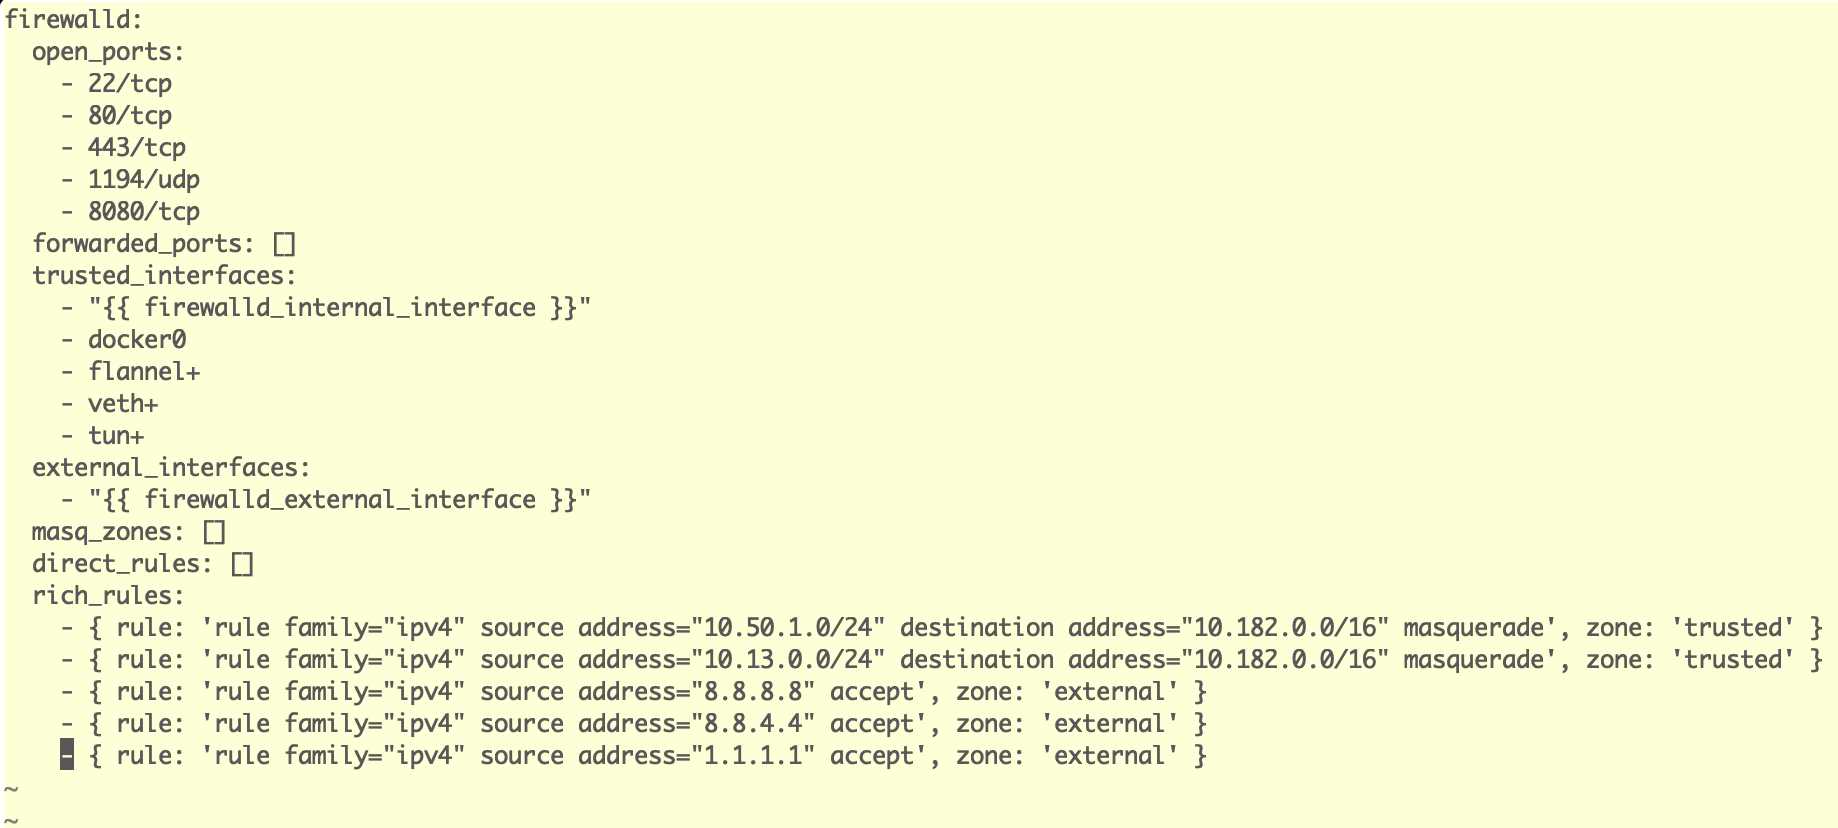
\includegraphics[height=6.3cm]{img/fwroleconfig}
\end{minipage}
\end{textblock*}
\end{frame}

\begin{frame}{\ \ \ Необходимость в модуле}
\setstretch{1.2}
\begin{textblock*}{\framewidth-0.8cm}(0.5cm,1.5cm)
\begin{itemize}
  \item {\color {darkpastelgreen}{\bf Я добавляю} правило, оно работает}
  \item {\color {darkpastelgreen}Я не заблокировал весь трафик (валидация)}
  \item {\color {darkpastelgreen}Нет противоречий (валидация)}
  \item {\color {darkpastelgreen}После перезагрузки система находится в известном состоянии}
  \item {\color {darkpastelgreen}Повторное применение не меняет состояние системы (идемпотентность)}
\end{itemize}
\end{textblock*}
\end{frame}

\begin{frame}{\ \ \ Необходимость в модуле}
\setstretch{1.2}
\begin{textblock*}{\framewidth-0.8cm}(0.5cm,1.5cm)
\begin{itemize}
  \item {\color {darkpastelgreen}{\bf Я удаляю} правило, оно удаляется}
\end{itemize}
\end{textblock*}
\end{frame}

\begin{frame}{\ \ \ Ansible модуль для firewalld}
\setstretch{1.2}
\begin{textblock*}{\framewidth-0.8cm}(0.5cm,1.5cm)
\begin{itemize}
  \item G(T/S)D
\end{itemize}
\begin{minipage}{\textwidth}
  \centering
  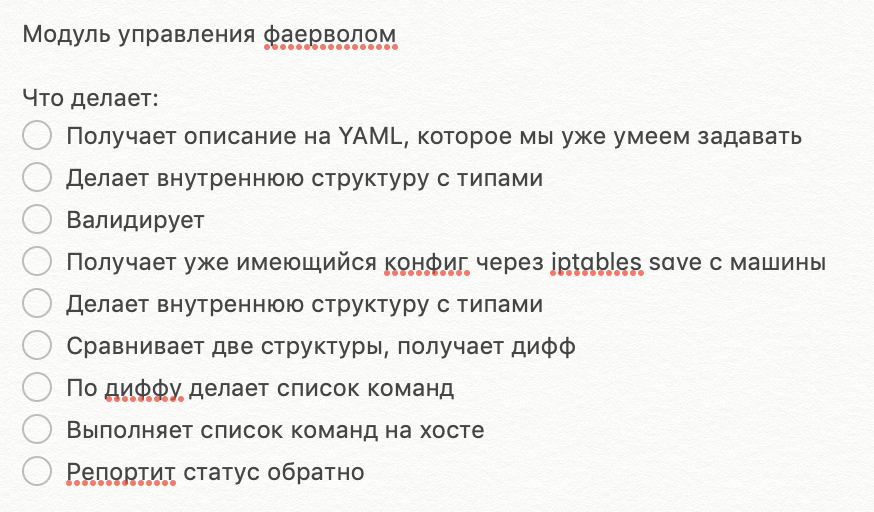
\includegraphics[height=6.3cm]{img/plan}
\end{minipage}
\end{textblock*}
\end{frame}

\begin{frame}{\ \ \ Ansible модуль для firewalld}
\setstretch{1.2}
\begin{textblock*}{\framewidth-0.8cm}(0.5cm,1.5cm)
\begin{itemize}
  \item Тот же формат конфигурации, что у роли
\end{itemize}
\end{textblock*}
\end{frame}

\begin{frame}{\ \ \ Ansible модуль для firewalld}
\setstretch{1.2}
\begin{textblock*}{\framewidth-0.8cm}(0.5cm,1.5cm)
\begin{itemize}
  \item Тот же формат конфигурации, что у роли
  \item Пишем на Haskell
\end{itemize}
\end{textblock*}
\end{frame}

\begin{frame}{\ \ \ Ansible модуль для firewalld}
\setstretch{1.2}
\begin{textblock*}{\framewidth-0.8cm}(0.5cm,1.5cm)
\begin{itemize}
  \item Тот же формат конфигурации, что у роли
  \item Пишем на Haskell
  \item Сейчас (кажется) готова заглушка для модуля, которая может принять параметры и
    вернуть обратно статус (всегда одинаковый)
\end{itemize}
\end{textblock*}
\end{frame}

\begin{frame}{\ \ \ Ansible модуль для firewalld}
\setstretch{1.2}
\begin{textblock*}{\framewidth-0.8cm}(0.5cm,1.5cm)
\begin{itemize}
  \item Тот же формат конфигурации, что у роли
  \item Пишем на Haskell
  \item Сейчас (кажется) готова заглушка для модуля, которая может принять параметры и
    вернуть обратно статус (всегда одинаковый)
  \item To be continued...
\end{itemize}
\end{textblock*}
\end{frame}

\begin{frame}{\ \ \ Выводы}
\setstretch{1.2}
\begin{textblock*}{\framewidth-0.8cm}(0.5cm,1.5cm)
\begin{itemize}
  \item Управление фаерволом - долго, дорого, неаккуратно
  \item Но мы, хотя бы, пытаемся
\end{itemize}
\end{textblock*}
\end{frame}

\begin{frame}{\ \ \ That's all, folks!}
\setstretch{1.2}
\begin{textblock*}{\framewidth-0.8cm}(0.5cm,1.5cm)
\begin{itemize}
  \item \href{mailto:alexclear@gmail.com}{\color{blue}{alexclear@gmail.com}}
  \item \href{https://telegram.me/lhommequipleure}{\color{blue}{https://telegram.me/lhommequipleure}}
  \item \href{https://telegram.me/demeliorator\_pod}{\color{blue}{https://telegram.me/demeliorator\_pod}}
\end{itemize}
\end{textblock*}
\end{frame}

\end{Large}

\end{document}
